\documentclass[a6paper, 12pt, parskip=half, DIV=14]{scrartcl}

\usepackage[dvipsnames]{xcolor}
\usepackage{tikz}

\usepackage{testpiece}
\usepackage{caption}
\usepackage{ragged2e}
% Minimize unwanted hyphenation
\tolerance=1
\emergencystretch=\maxdimen
\hyphenpenalty=1
\hbadness=10000

\usepackage{fontspec}
\setmainfont{Tex Gyre Schola}
%\setmainfont{Qwigley}

\usepackage{eso-pic}
\usepackage{booktabs}

%\definecolor{SunriseBlue}{HTML}{A9C2E5}
\setkomafont{section}{\setmainfont{Tex Gyre Schola}\LARGE\color{redfabric}\bfseries\scshape}
\setkomafont{subsection}{\setmainfont{Tex Gyre Schola}\Large\color{redfabric}\bfseries\scshape}
\setkomafont{subsubsection}{\setmainfont{Tex Gyre Schola}\large\color{redfabric}\bfseries\scshape}

% Adjust spacing before and after section headings
\RedeclareSectionCommand[
  runin=false,
  beforeskip=1.0\baselineskip,
  afterskip=-0.0\baselineskip
]{section}

% Adjust spacing before and after subsection headings
\RedeclareSectionCommand[
  runin=false,
  beforeskip=1.0\baselineskip,
  afterskip=-0.0\baselineskip
]{subsection}

% Adjust spacing before and after subsubsection headings
\RedeclareSectionCommand[
  runin=false,
  beforeskip=1.0\baselineskip,
  afterskip=-0.0\baselineskip
]{subsubsection}


\usepackage{enumitem}
\setlist[description]{labelindent=0pt, labelsep=\widthof{ }, leftmargin=\widthof{\textbf{License: }}, font=\setmainfont{Tex Gyre Schola}\bfseries}

\usepackage[hang,flushmargin]{footmisc}
\newcommand\blfootnote[1]{%
  \begingroup
  \renewcommand\thefootnote{}\footnote{#1}%
  \addtocounter{footnote}{-1}%
  \endgroup
}

\renewcommand{\thefootnote}{\fnsymbol{footnote}}
\renewcommand{\footnoterule}{%
  \kern -3pt
  \hrule width \textwidth height 0.5pt
  \kern 2pt
}

\usepackage[hidelinks]{hyperref}
\usepackage[type={CC}, version={4.0}, modifier={by-sa}]{doclicense} % Add text and icons for creative commons license
%\usepackage{array}

\raggedright
\pagestyle{empty}
\begin{document}

\begin{titlepage}
\AddToShipoutPictureBG{
\begin{tikzpicture}[remember picture, overlay]
%	\node () at (current page.center) {\includegraphics[width=\pagewidth, height=\pageheight]{Images/aloft_cover_background.png}};
	\node () at (current page.center) {\includegraphics[width=\pagewidth, height=\pageheight]{Images/test_piece_cover.png}};
\end{tikzpicture}
}

\enlargethispage{3.5\baselineskip}
\Large
\setmainfont[Scale=1.05]{Playball}
\phantom{test}
\vfill
\begin{center}
\begin{tikzpicture}
\node[draw, black, ultra thick, fill=brass, rounded corners=3mm, text width = 75mm, align=center, text height=2.25ex] at (0,0) {\textcolor{black}{Designed by Michael Purcell}};
\end{tikzpicture}
\end{center}
%\normalsize
%\phantom{a}
\end{titlepage}


\ClearShipoutPicture
\enlargethispage{1.75\baselineskip}
\section*{Overview}
Test Piece is a two-player card-drafting game about British-style brass bands. It can be played in about thirty minutes and is intended for players who are at least twelve years old.

During the game, you will assume the roles of rival music directors who are competing to build the best band from a limited pool of local musicians.

\vspace{0.1cm}

\begin{figure}[h]
\centering
%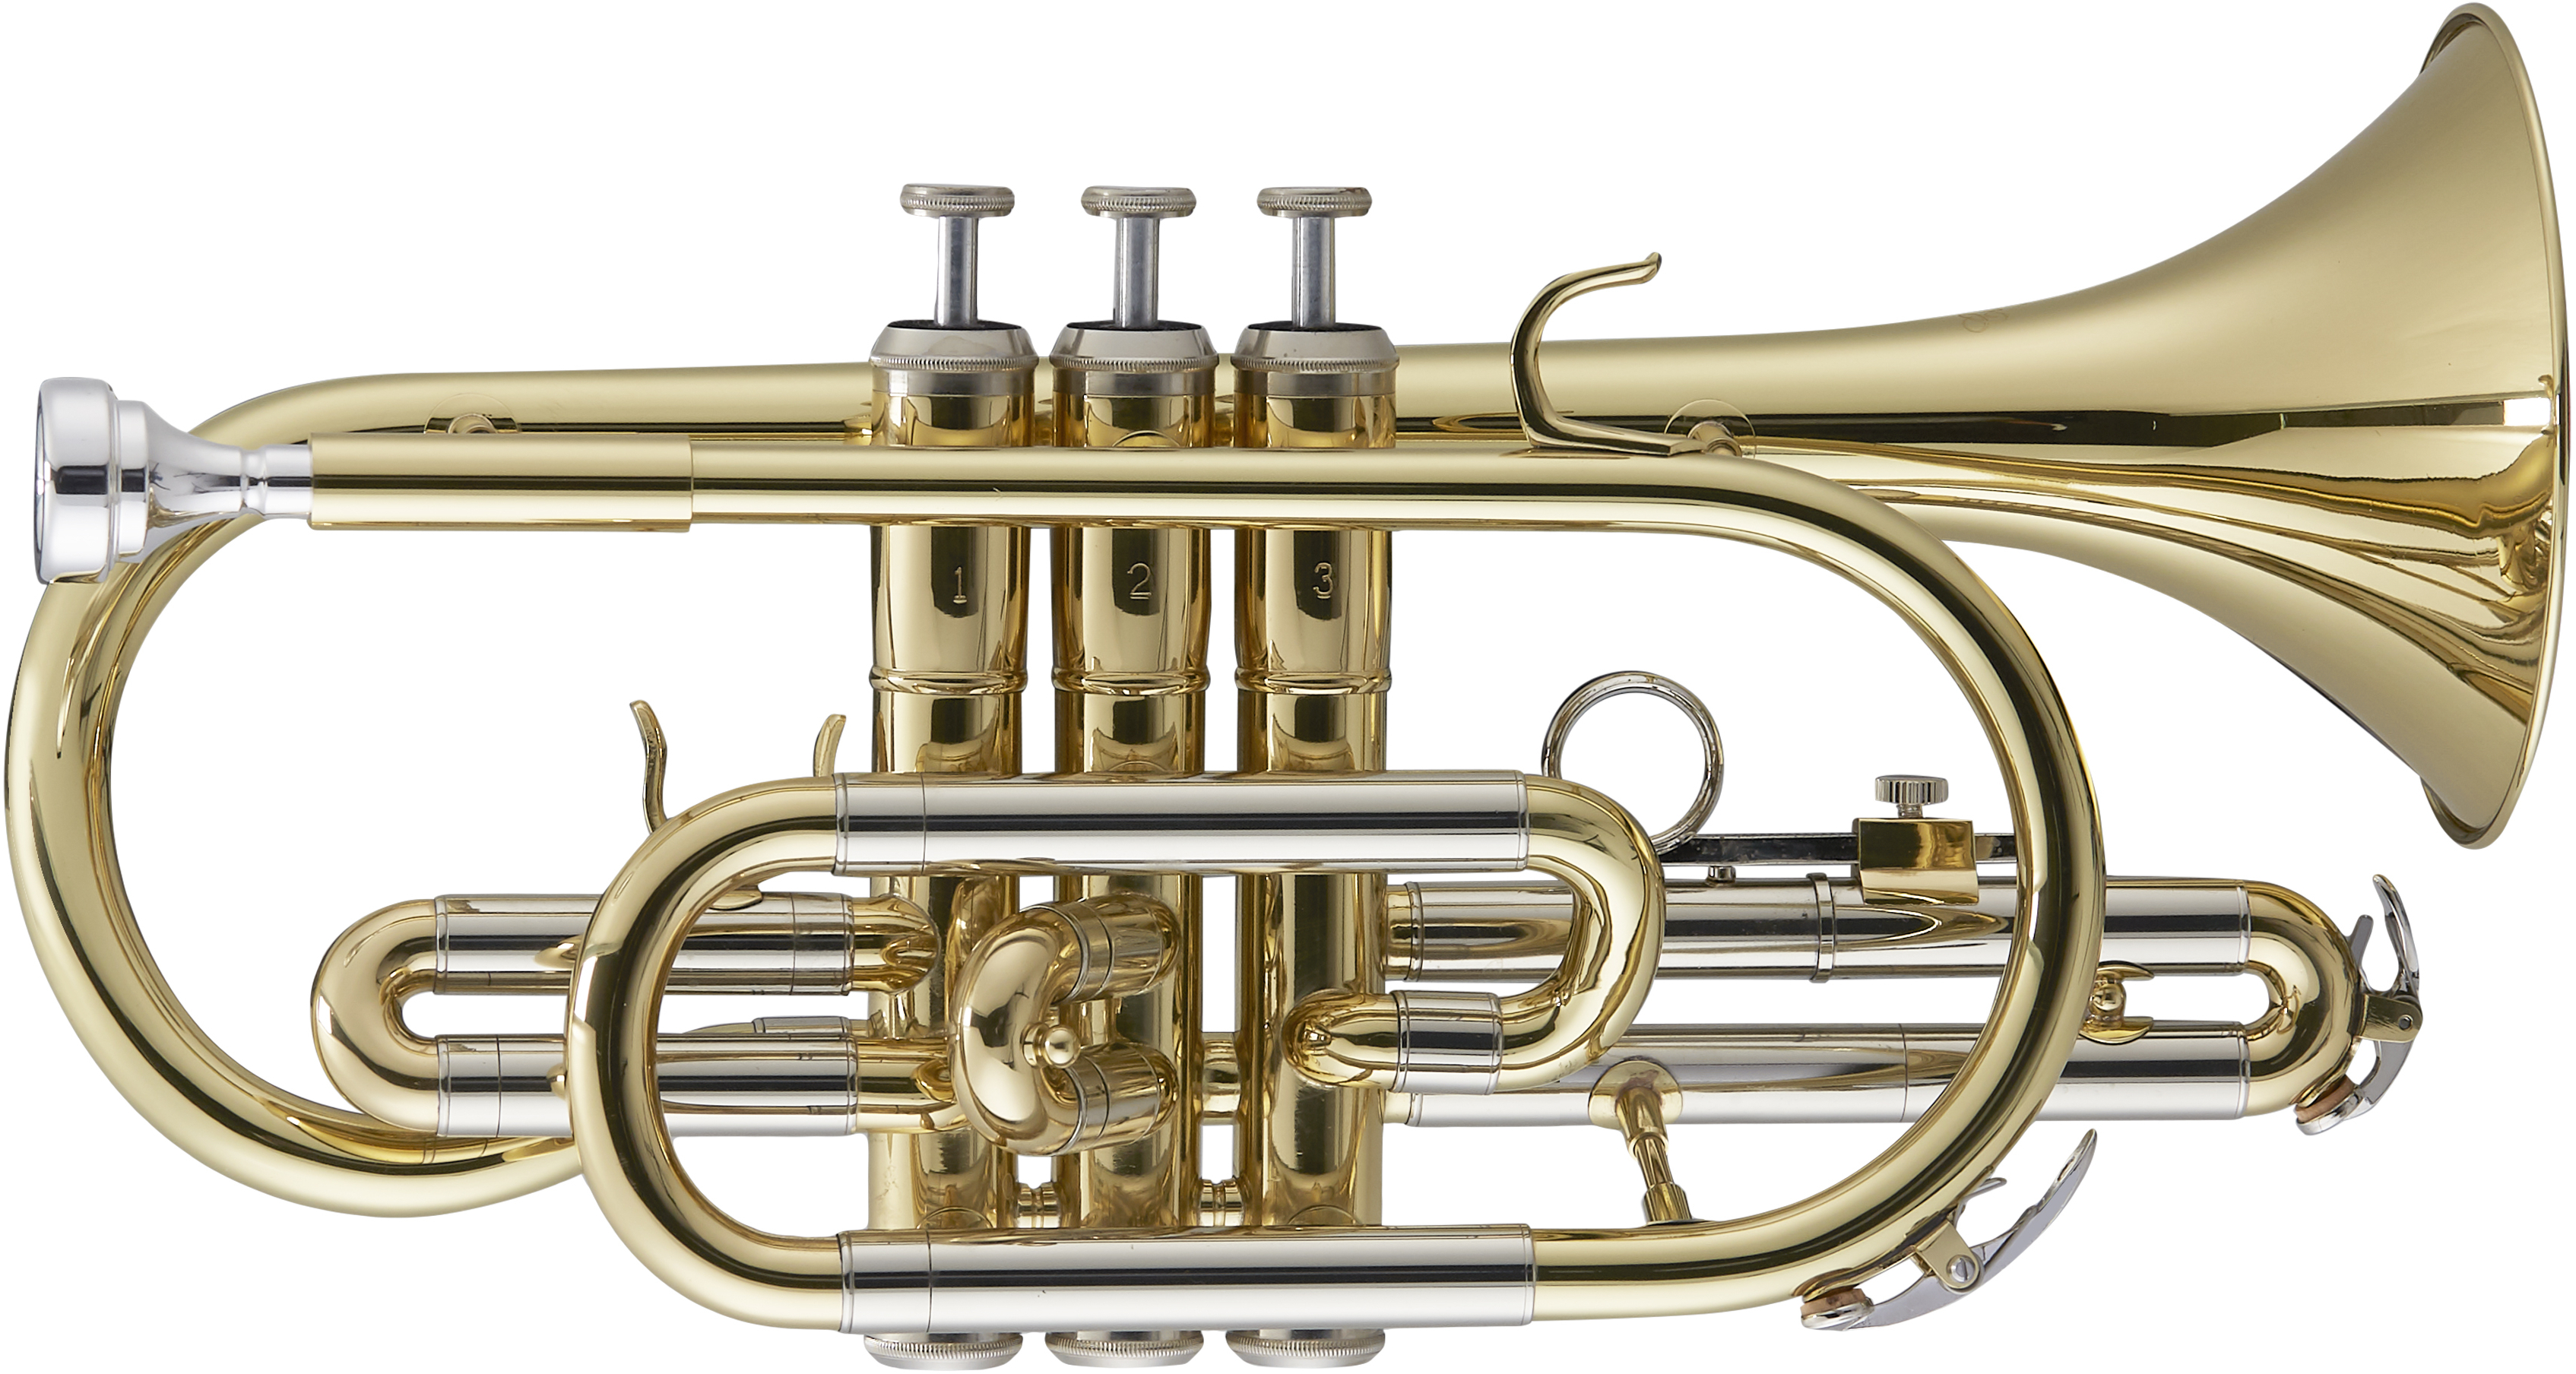
\includegraphics[width=7cm]{Images/shutterstock_cornet.jpg}
%\includegraphics[height=4.75cm, rotate=-15]{Images/shutterstock_tuba.jpg}
%\quad
%\includegraphics[height=4.75cm, rotate=-15]{Images/shutterstock_tuba.jpg}
    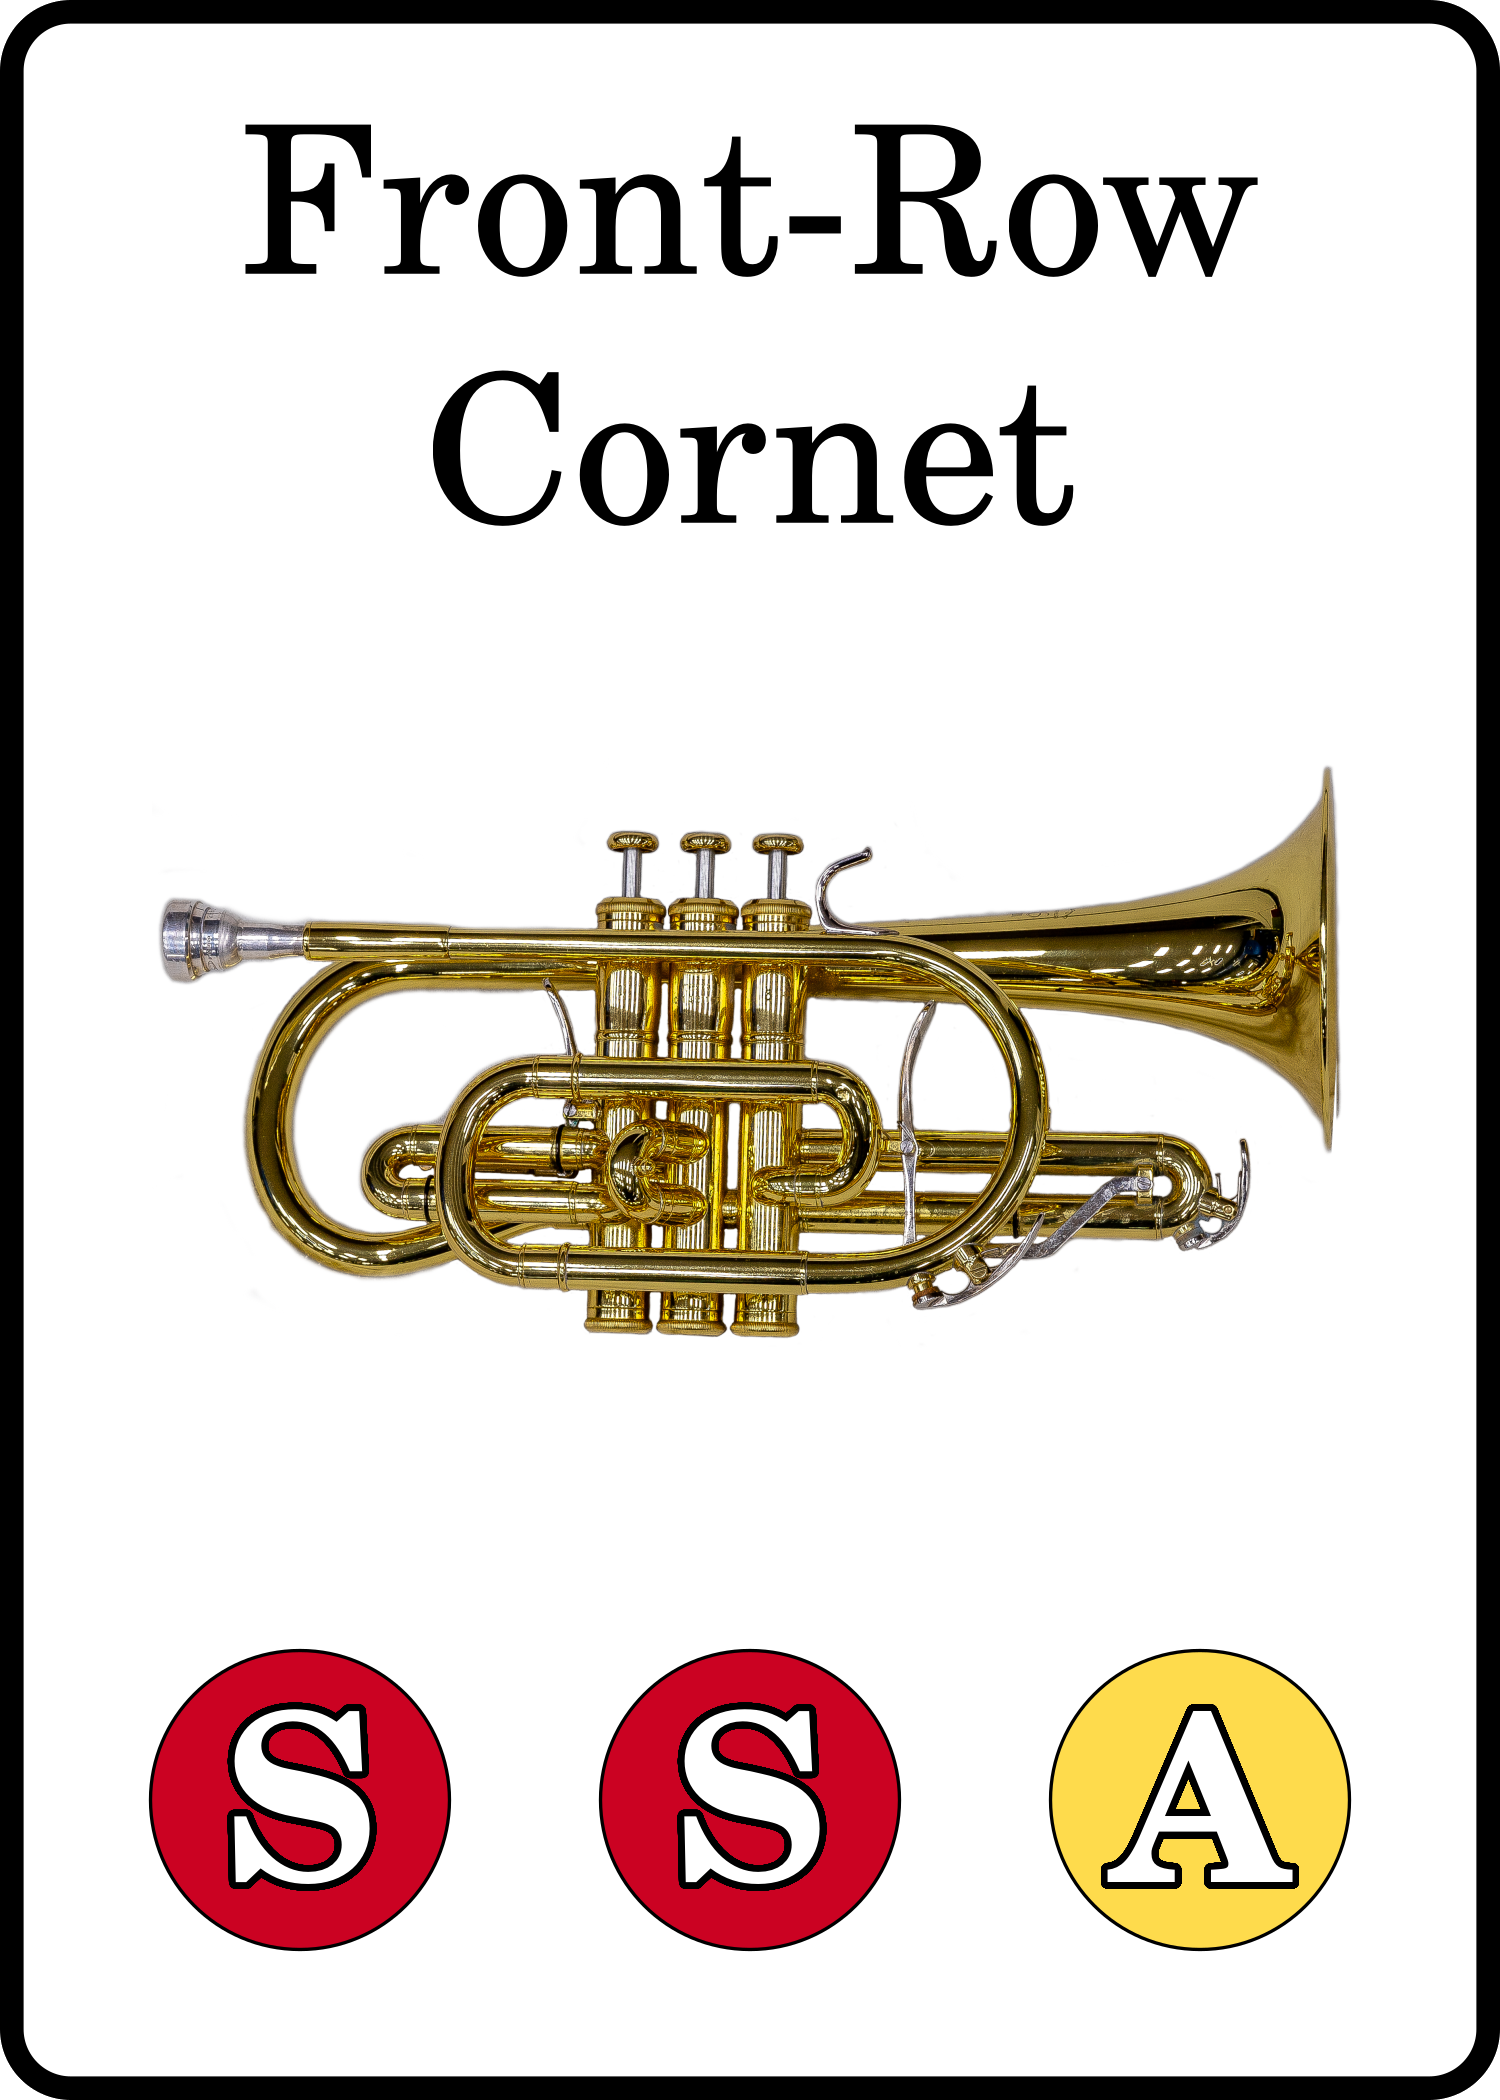
\includegraphics[scale=0.065]{Images/CardImages/cornet_display_front.png}
    \qquad
    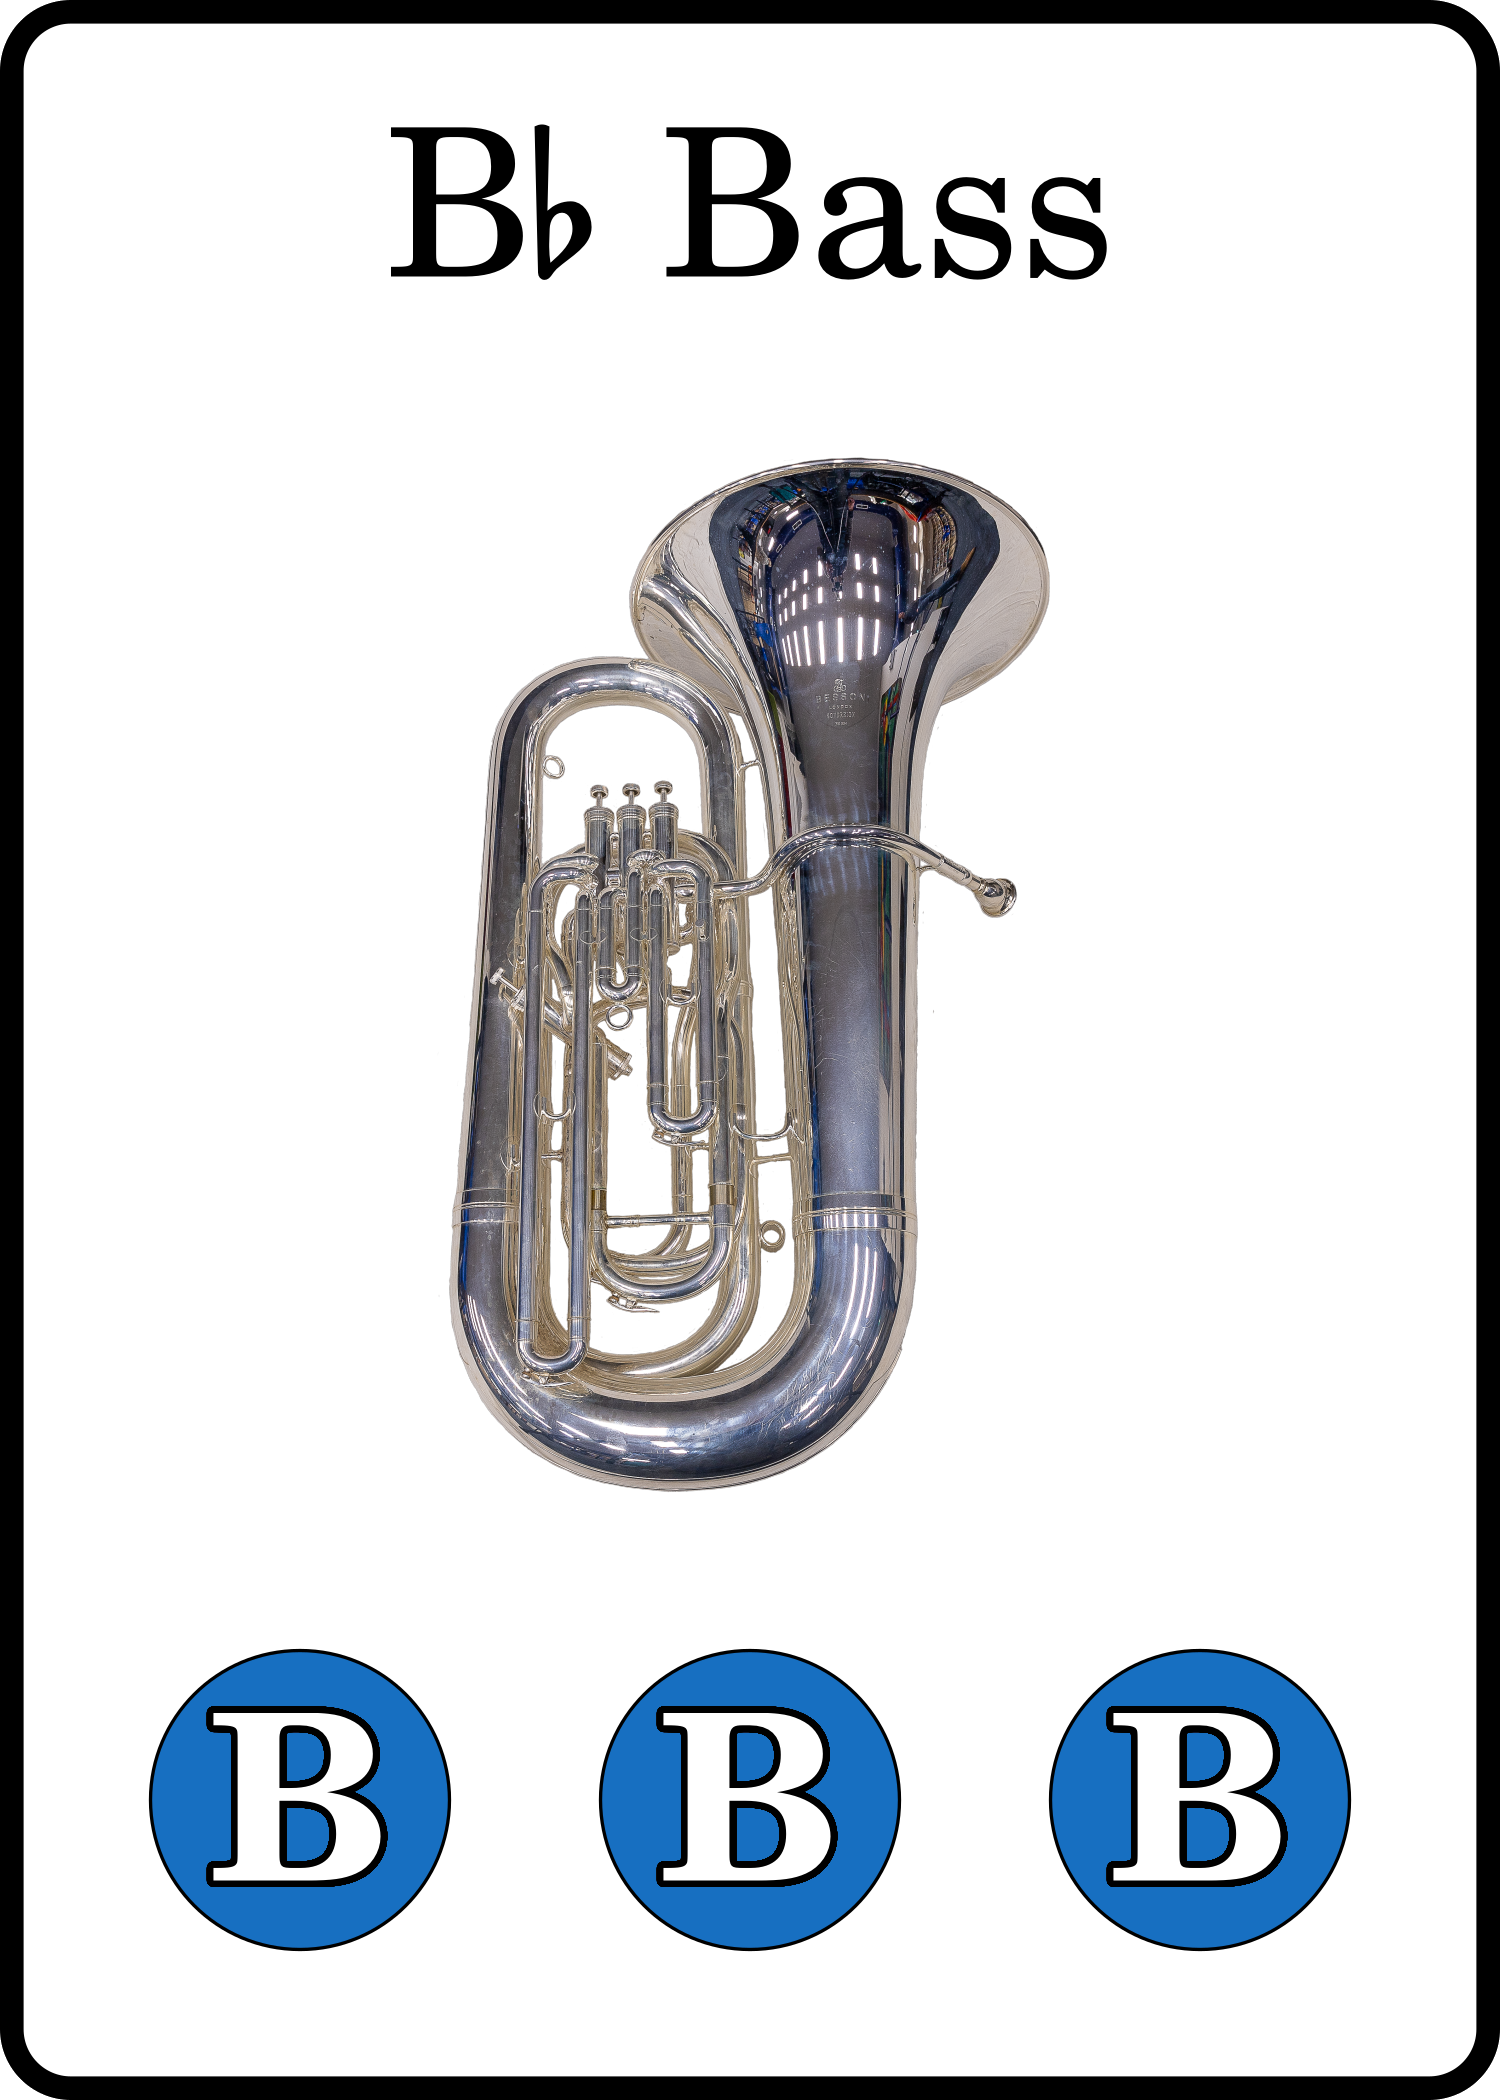
\includegraphics[scale=0.065]{Images/CardImages/bass_display_front.png}
	\caption*{Instrument cards that represent two of the instruments played by local musicians.}
\end{figure}

\newpage
\enlargethispage{1.75\baselineskip}

\section*{Components}
\begin{itemize}[leftmargin=4ex, nosep]
  \item 36 instrument cards
%  	\vspace{-1ex}
    \begin{itemize}[nosep, leftmargin=*]
      \item 18 silver-backed cards
      \item 18 gold-backed cards
    \end{itemize}
    \begin{figure}[h]
	\centering    
    
\includegraphics[scale=0.04]{Images/CardImages/silver_display_back.png}
    \qquad
    
\includegraphics[scale=0.04]{Images/CardImages/gold_display_back.png}
\end{figure}
  \item 8 pawns
    \begin{figure}[h]
	\centering    
    
\includegraphics[scale=0.3]{Images/pawn_red.png}
    
\includegraphics[scale=0.3]{Images/pawn_yellow.png}
    
\includegraphics[scale=0.3]{Images/pawn_green.png}
    
\includegraphics[scale=0.3]{Images/pawn_blue.png}
	\qquad
	
\includegraphics[scale=0.3]{Images/pawn_red.png}
    
\includegraphics[scale=0.3]{Images/pawn_yellow.png}
    
\includegraphics[scale=0.3]{Images/pawn_green.png}
    
\includegraphics[scale=0.3]{Images/pawn_blue.png}

    \end{figure}
  \item 2 score boards
  \begin{figure}[h]
  \centering
  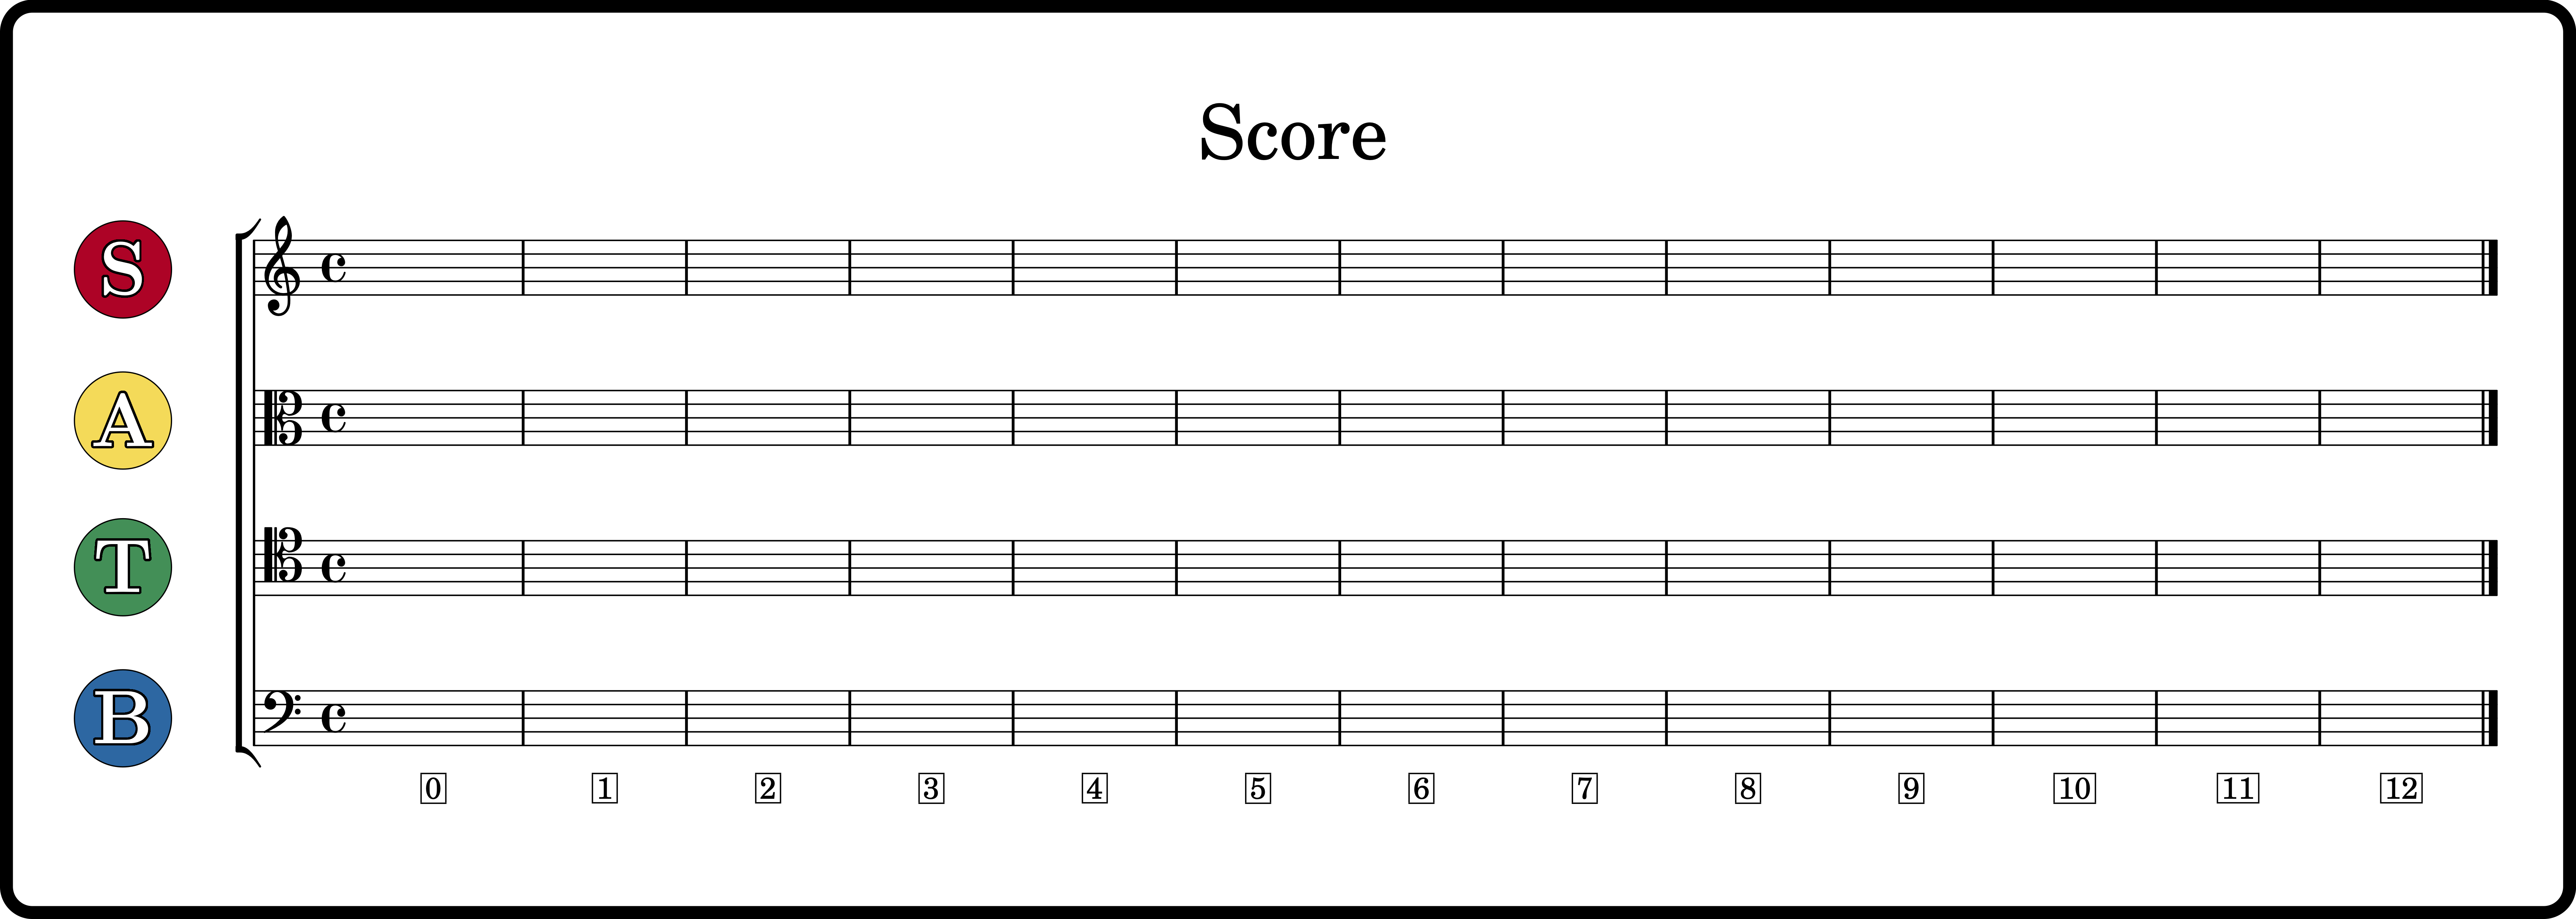
\includegraphics[width=\textwidth]{Images/score_board_diagram_thin_border.png}
  \end{figure}
\end{itemize}


\newpage
\enlargethispage{1.75\baselineskip}
\section*{Set Up}
\begin{enumerate}[leftmargin=4ex]
  \item Separate the two decks (silver-backed and gold-backed) of instrument cards. 
  \item Shuffle each deck of instrument cards.
  \item Combine the two instrument decks by placing one on top of the other.
  \item Place the combined instrument decks face down to one side of the play area.
  \item Place the score boards near the play area, one in front of each player.
  \item Place a pawn on Measure 12 (the rightmost position) of each row on both score boards. 
  \item Randomly determine who will be Player A and who will be Player B.
\end{enumerate}

\vspace{0.25cm}

\begin{figure}[h]
\centering
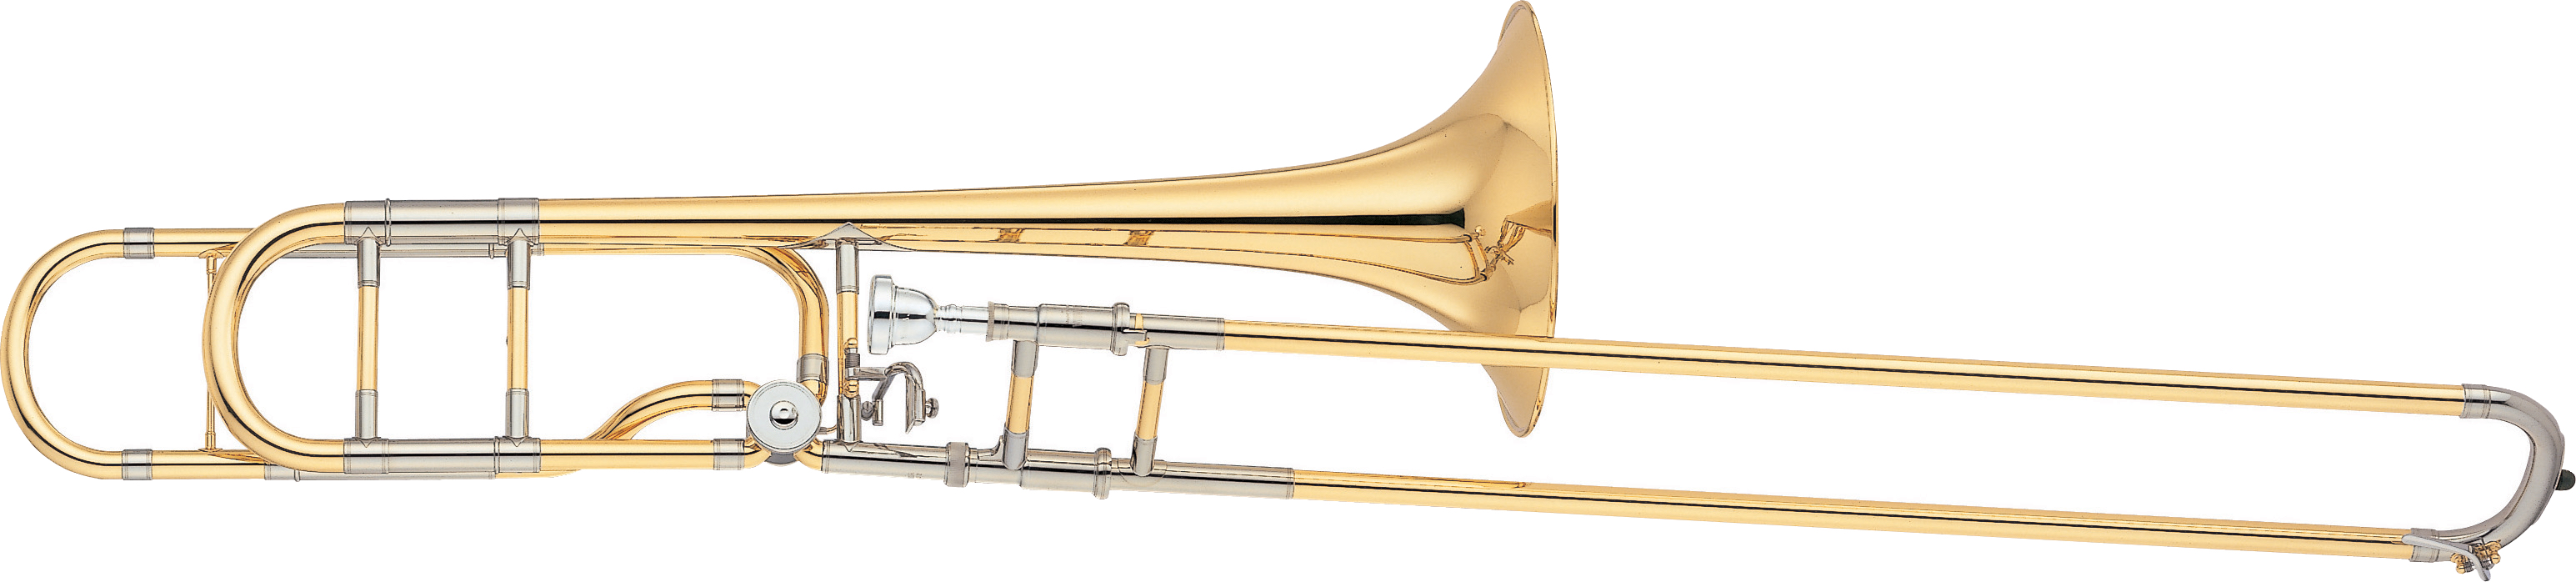
\includegraphics[width=7cm]{Images/wikipedia_trombone.jpg}
\end{figure}


\newpage
\enlargethispage{1.75\baselineskip}
\section*{Gameplay}
During the game, you will \emph{draft} instrument cards. You will add the cards that you draft to a grid of four rows and four columns called your \emph{tableau}.

The game consists of four \emph{rounds}. As you play, you will build eight \emph{performances}.
You will evaluate each performance for its merits in each of the four different \emph{voices}: Soprano, Alto, Tenor, and Bass.
{

\begin{figure}[h]
\centering
\Huge
\tikz{\pic {soprano}} \ \ \tikz{\pic {alto}} \ \ \tikz{\pic {tenor}} \ \ \tikz{\pic {bass}}
\caption*{The four voice symbols.}
\end{figure}
}
The game ends at the end of the fourth round. Your \emph{overall score} is the minimum of your scores for the four voices.

The player with the highest overall score wins the game. In the case of a tie, you should compare your next lowest voice scores in to determine the winner. 

\newpage
\enlargethispage{1.75\baselineskip}
\subsection*{Round Structure}
During each round, you should
\begin{enumerate}[leftmargin=4ex]
\item Place the top nine cards from the instrument deck face up in the middle of the play area. This is the \emph{draft row}.

\item Take turns drafting cards from the draft row. See \textcolor{redfabric}{\textbf{\scshape{Drafting}}} for details.

\item After you have drafted four cards, score your column performance for the round. See \textcolor{redfabric}{\textbf{\scshape{Scoring}}} for details.

\item Discard the last card in the draft row.
\end{enumerate}

At the end of the fourth round, score all four of your row performances.

\subsection*{First Player}
\begin{itemize}[leftmargin=4ex]
\item Player A will be the first player in Round 1 and Round 4.
\item Player B will be the first player in Round 2 and Round 3.
\end{itemize}

\newpage
\enlargethispage{1.75\baselineskip}
\subsection*{Drafting}
To draft a card, take that card from the draft row and place it in your tableau.
\begin{itemize}[leftmargin=4ex]
\item Place all of the cards that you draft in a given round in the same column.
% of your tableau.
\item Place each card that you draft in the bottom-most unoccupied position in the current column.
\end{itemize}

\subsection*{Turn Order}
Take turns drafting cards from the draft row as follows:
\begin{enumerate}[leftmargin=4ex]
\item The first player drafts one card.
\item The second player drafts two cards.
\item The first player drafts two cards.
\item The second player drafts two cards.
\item The first player drafts one card.
\end{enumerate}


\newpage
\enlargethispage{1.75\baselineskip}
\section*{Scoring}
A performance consists of four cards in one row or column of your tableau.

To score a performance:
\begin{enumerate}[leftmargin=4ex]
\item Count how many of each of the four voice symbols appear on its constituent cards. These are the performance's \emph{counts}.

\item Compute the difference between each performance count and the \emph{target value} of 3. These are the \emph{errors}.

\item Decrease your score for each voice by the size (absolute value) of its error.
\end{enumerate}

\vspace{0.5cm}

\begin{figure}[h]
\centering
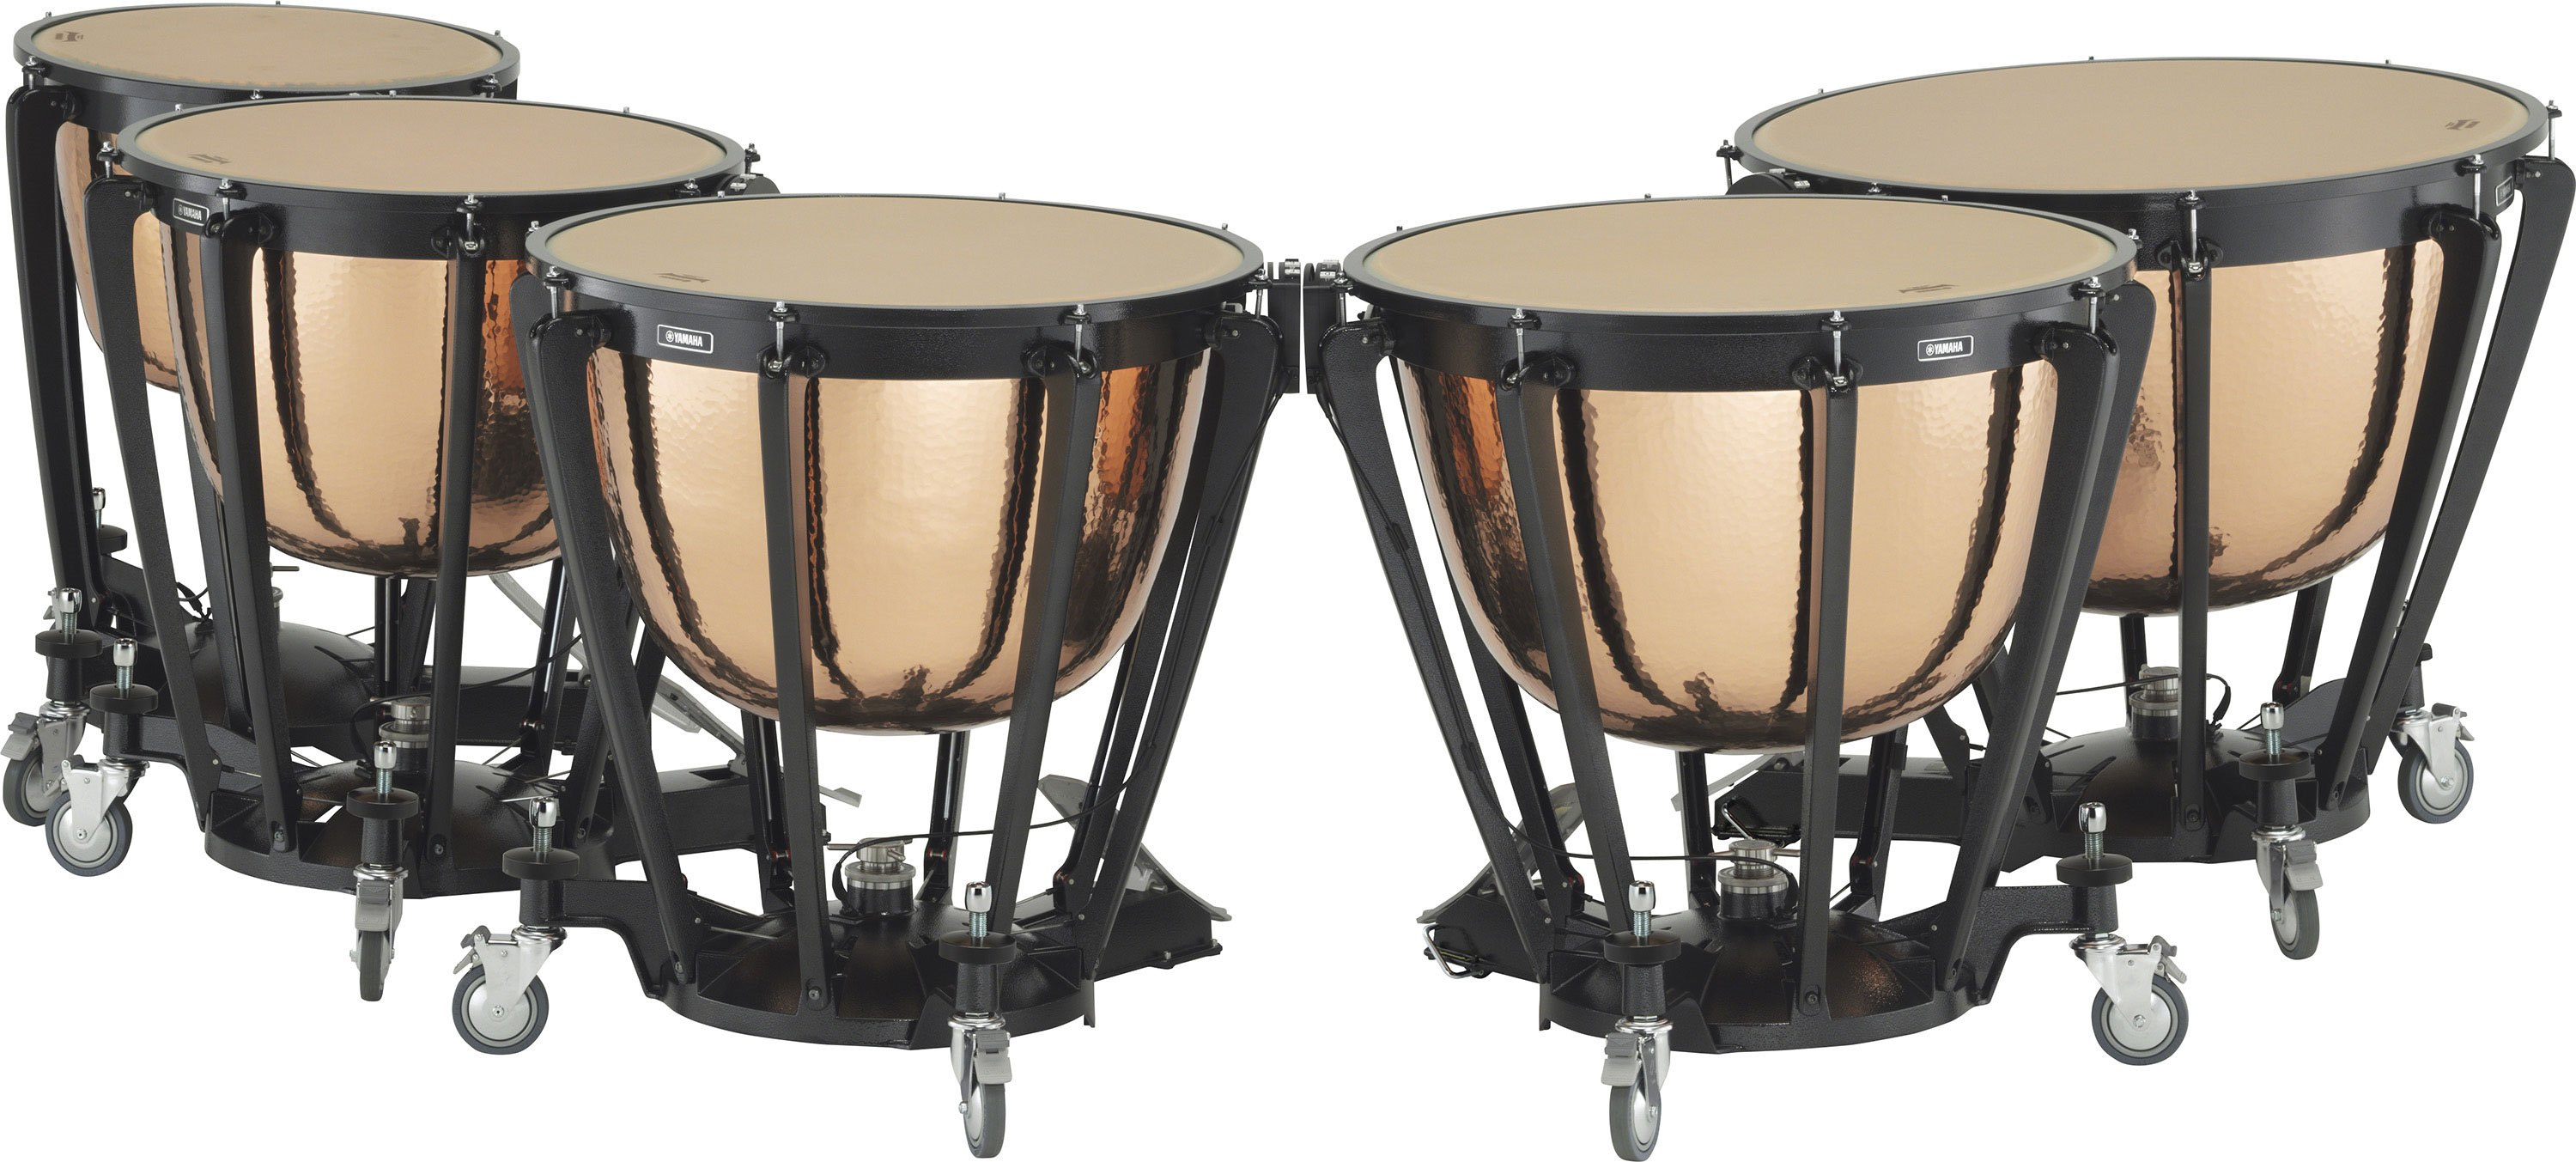
\includegraphics[width=7cm]{Images/yamaha_timpani.jpg}
\end{figure}

\newpage
\enlargethispage{1.75\baselineskip}
\subsection*{Example}
Consider a performance comprised of the four instrument cards depicted below.
\begin{figure}[h]
\centering
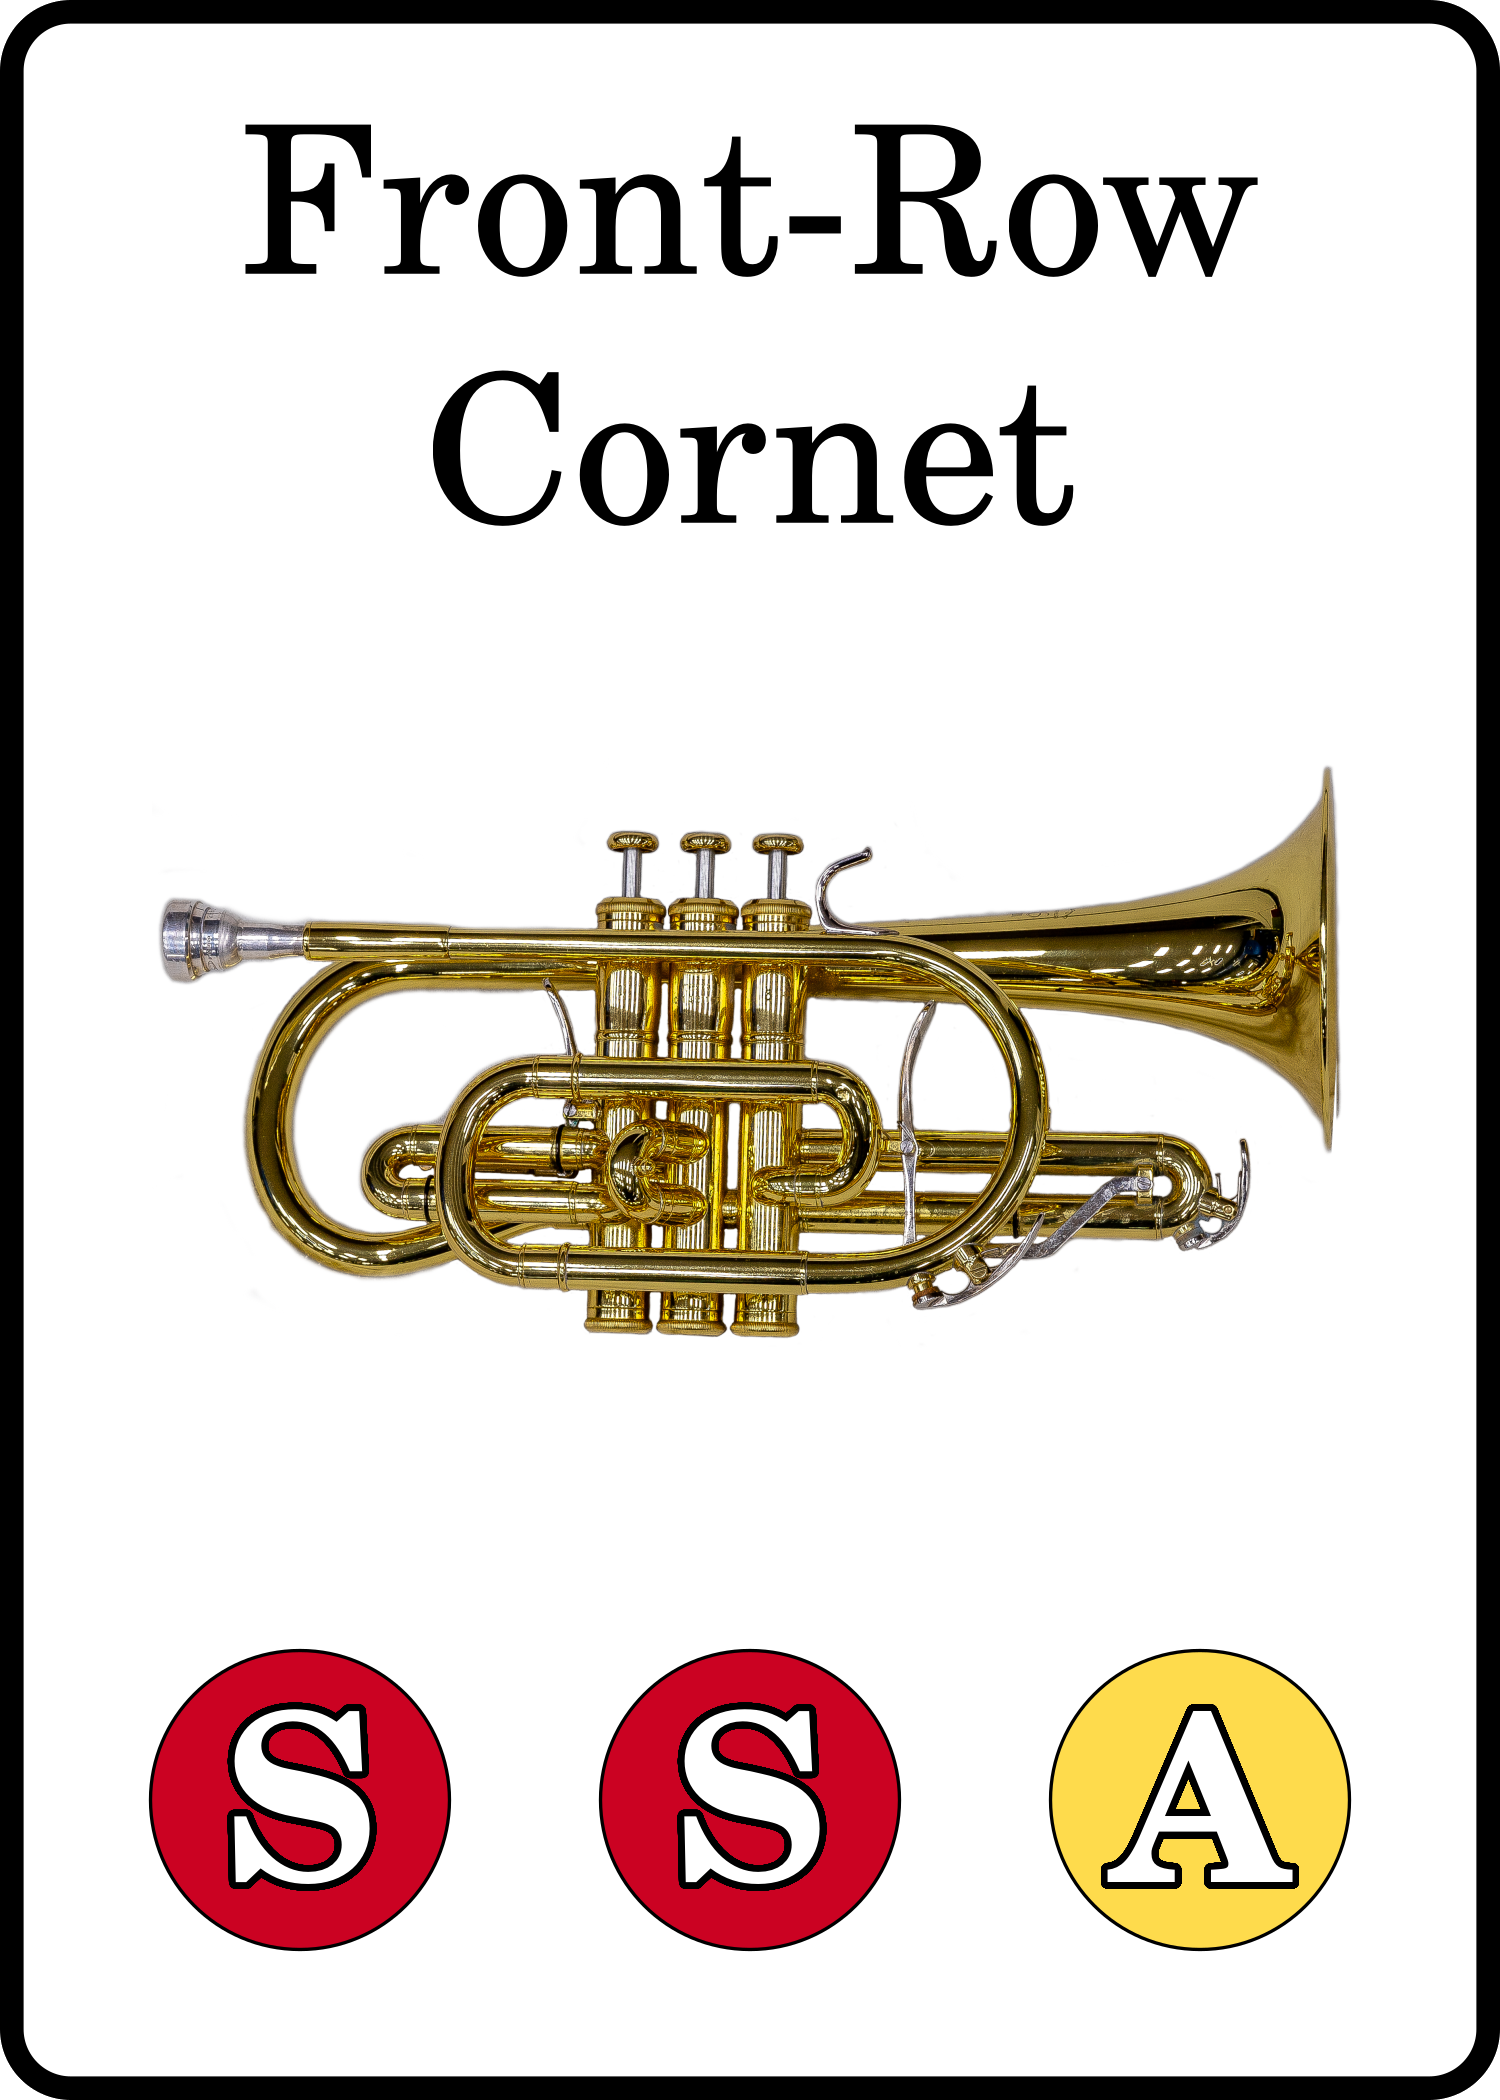
\includegraphics[scale=0.035]{Images/CardImages/cornet_display_front.png}
\ 
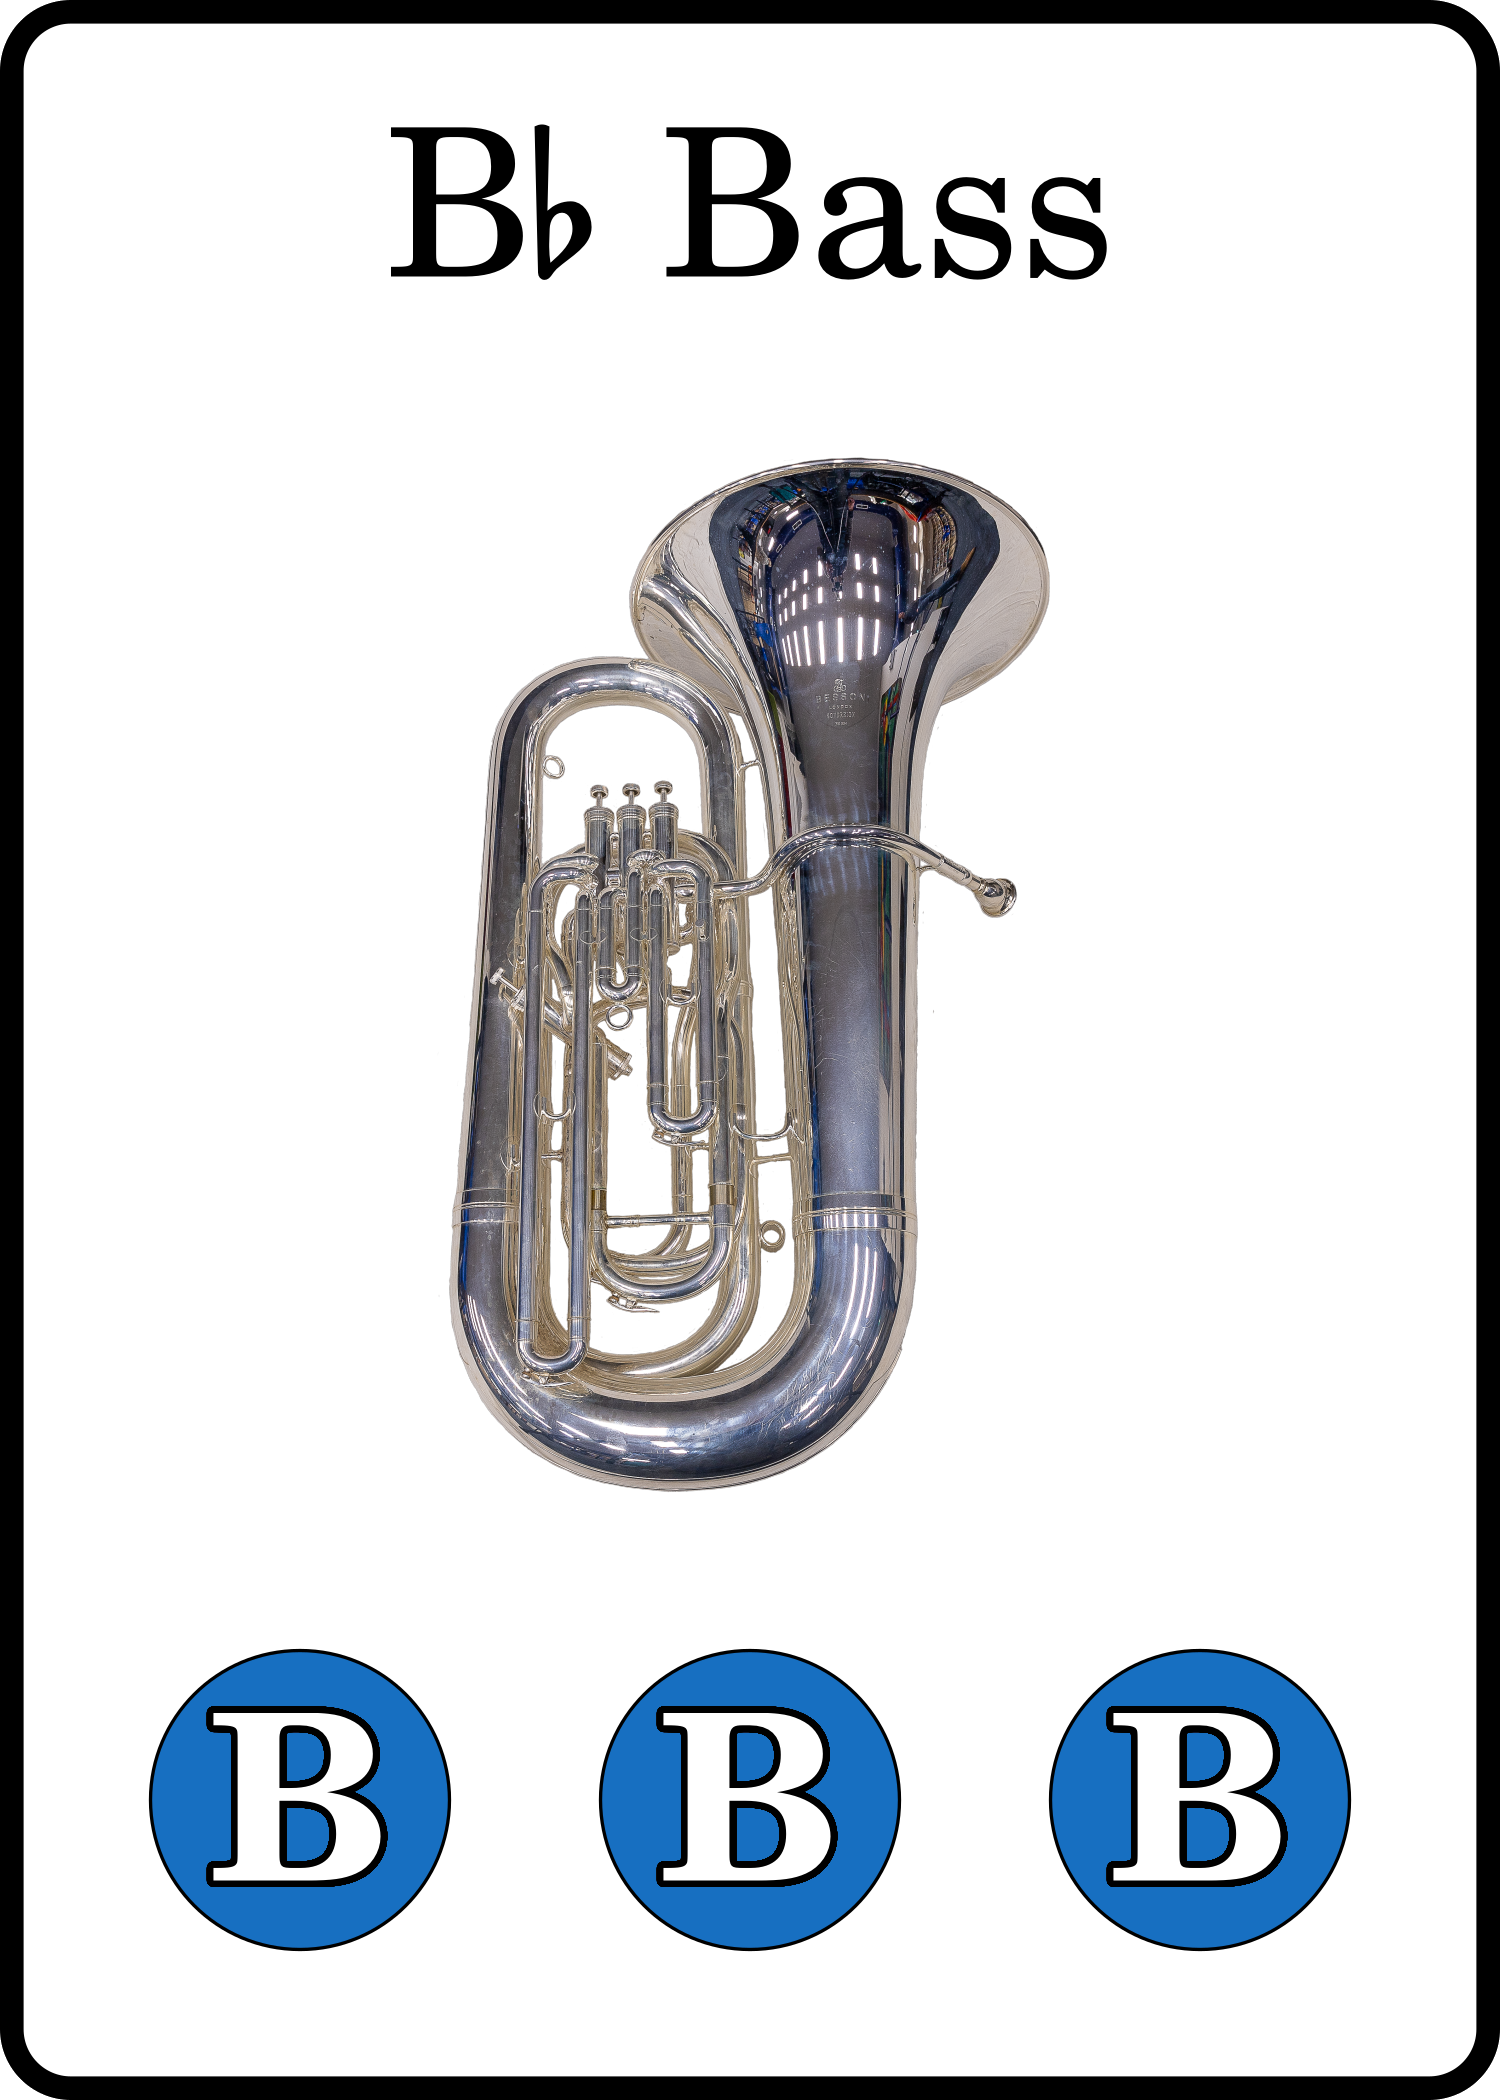
\includegraphics[scale=0.035]{Images/CardImages/bass_display_front.png}
\ 
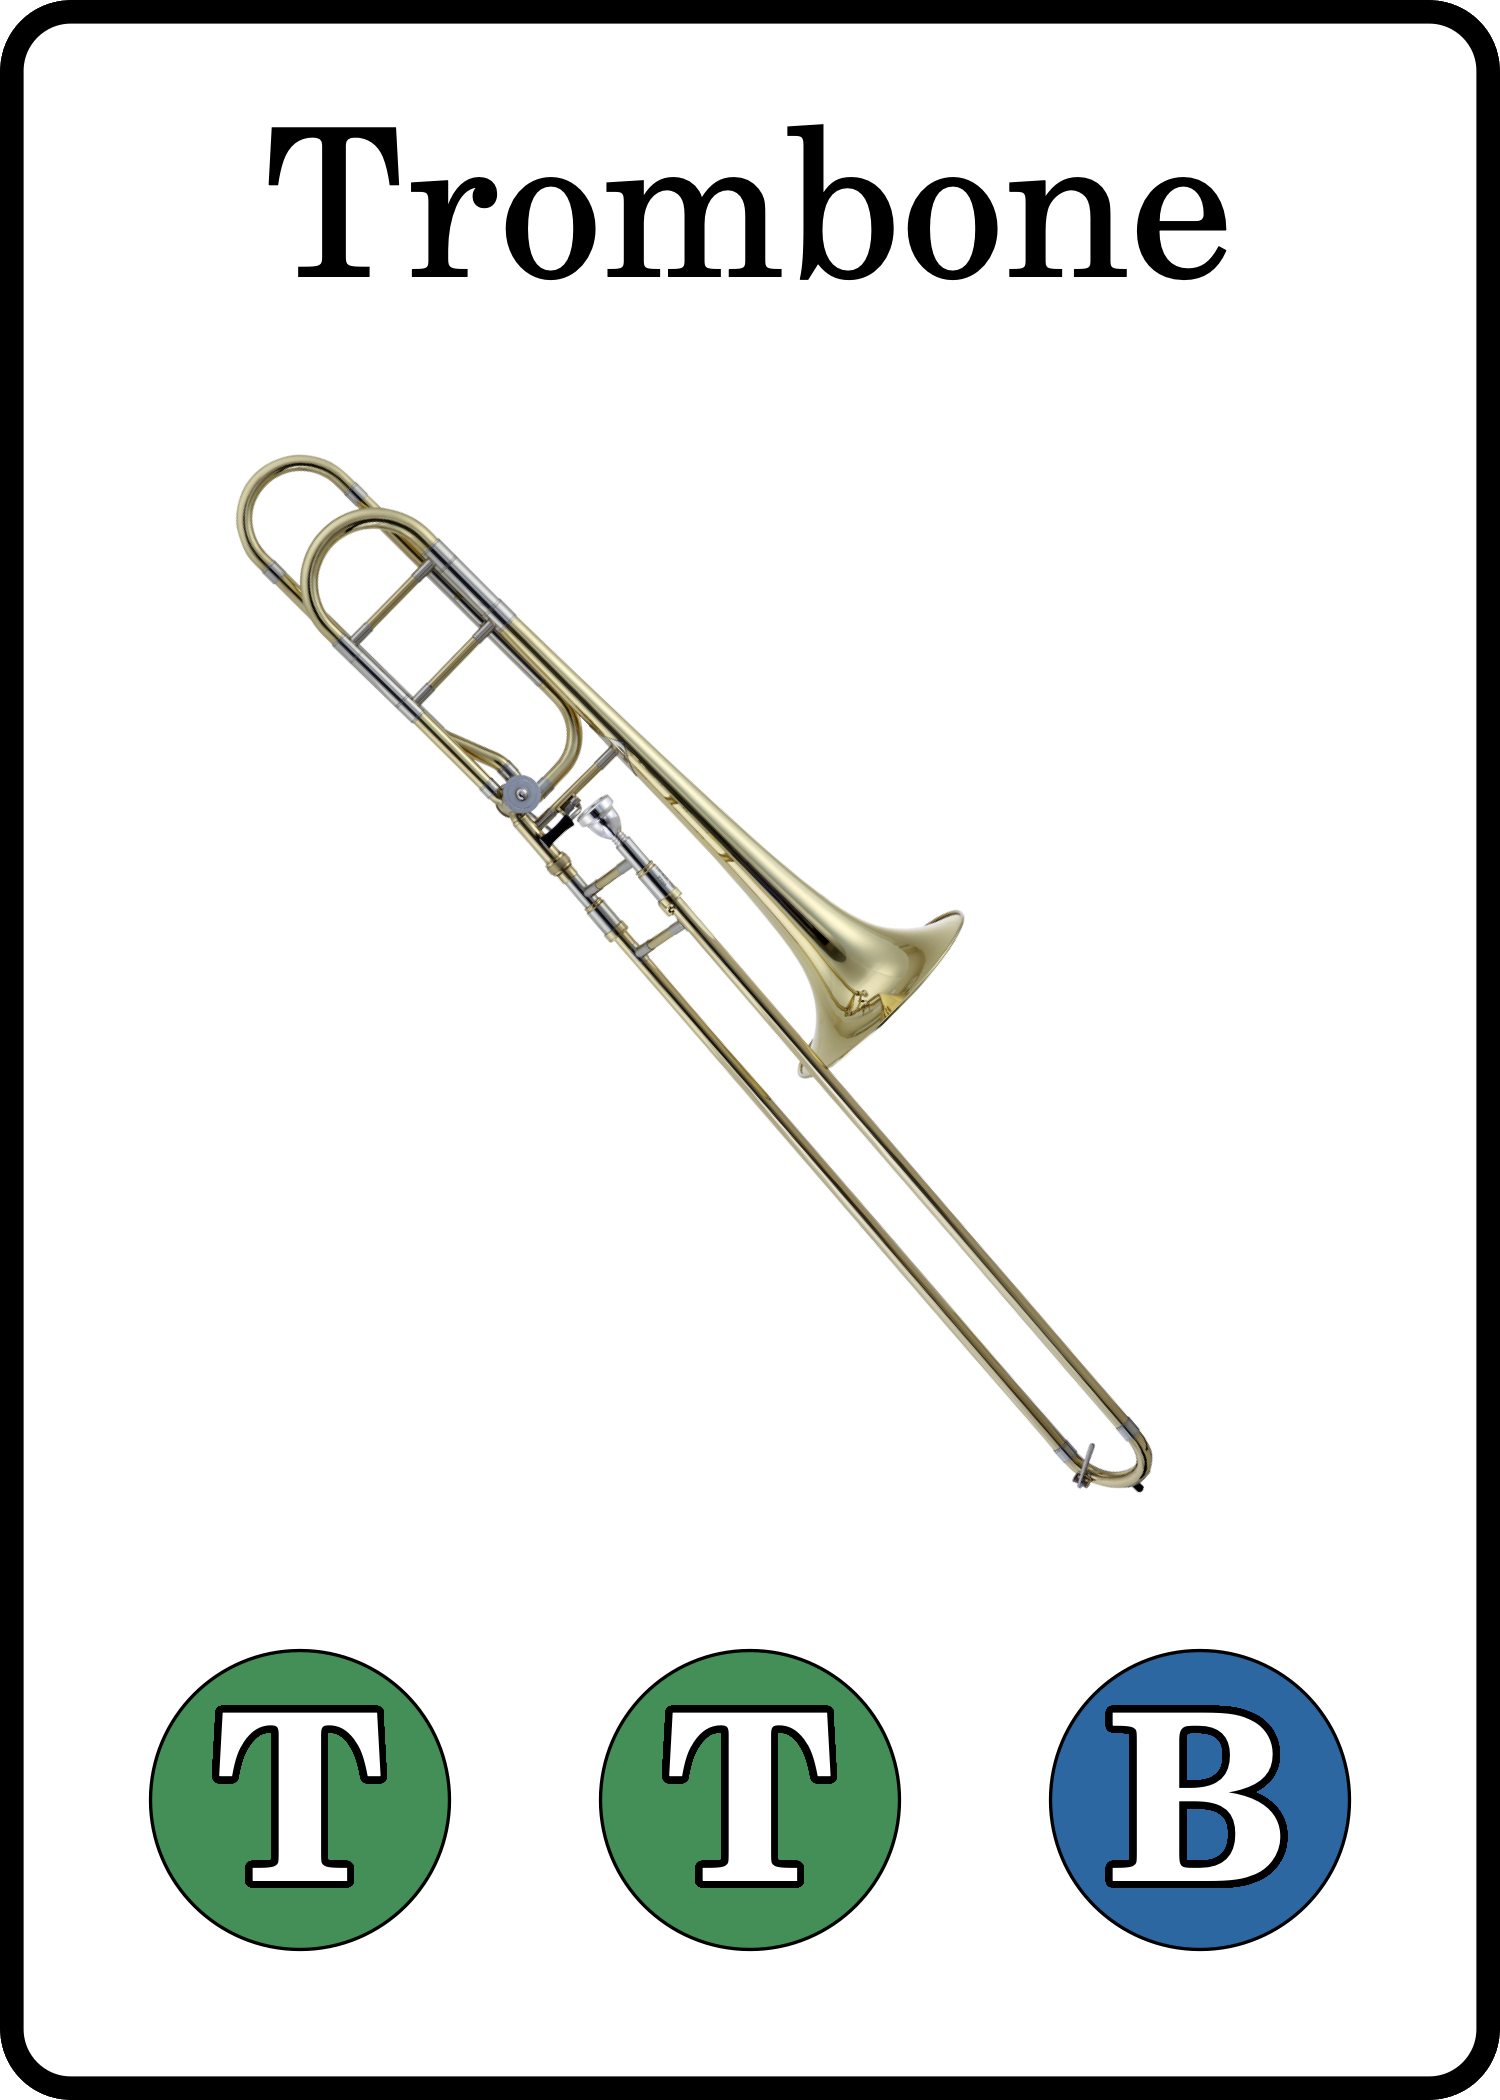
\includegraphics[scale=0.035]{Images/CardImages/trombone_display_front.png}
\ 
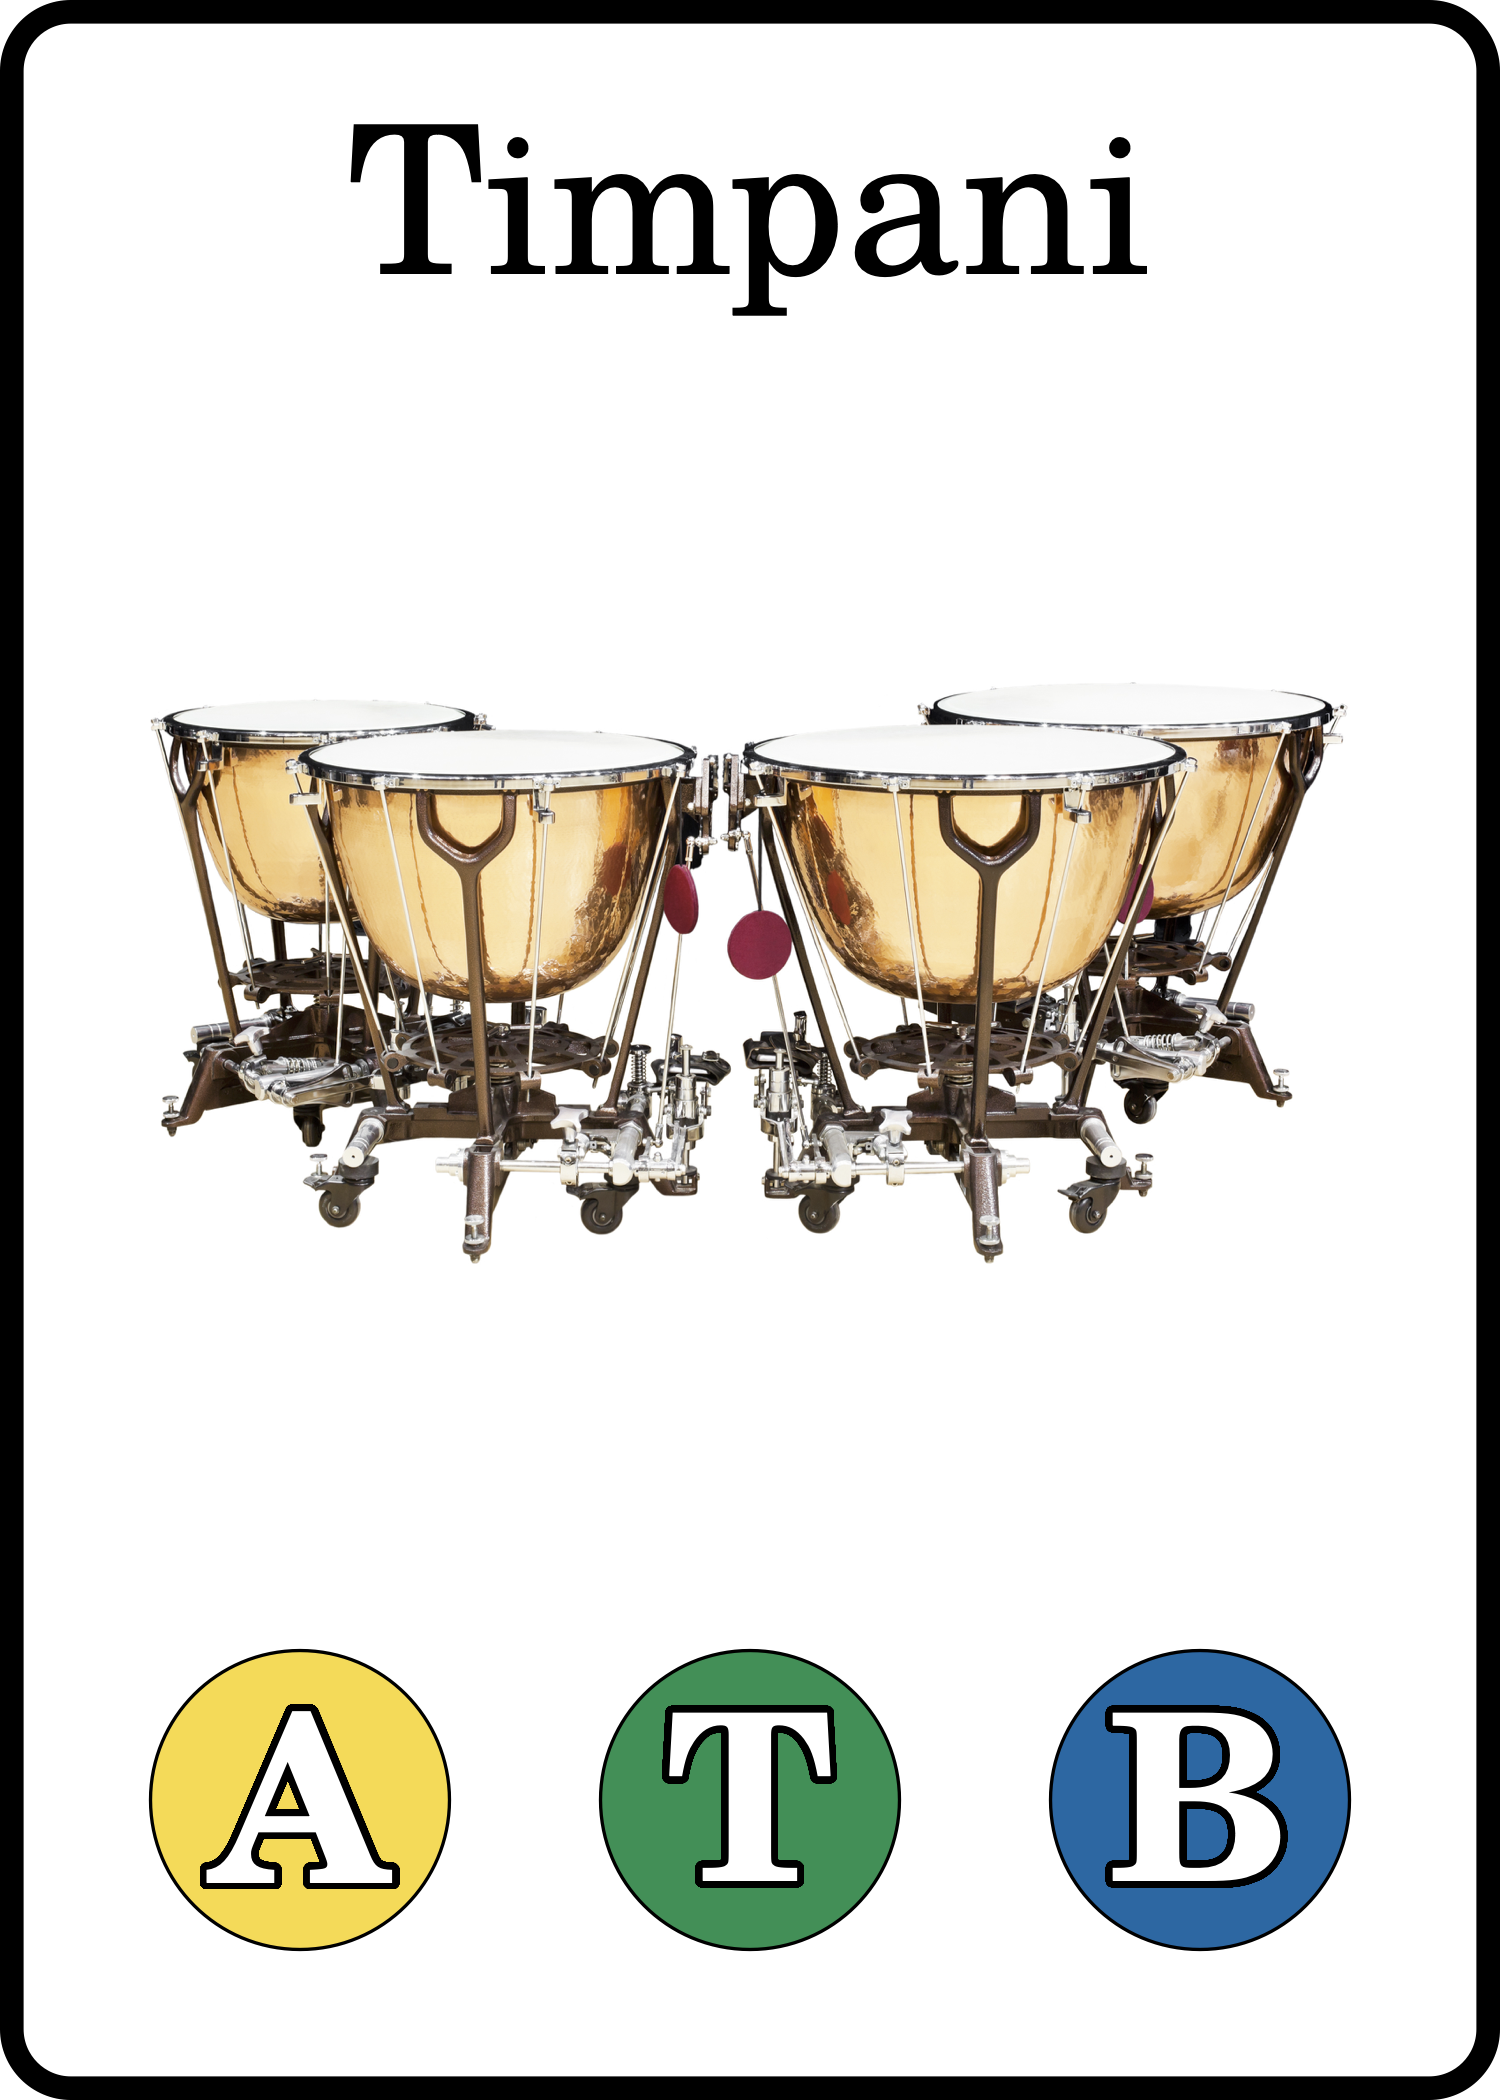
\includegraphics[scale=0.035]{Images/CardImages/timpani_display_front.png}
%\caption*{Instrument cards that represent two of the instruments played by local musicians.}
\end{figure}

To score this performance, we compute its counts, errors, and penalties as follows:
\begin{table}[h]
\centering
\begin{tabular}{lcccc}\toprule
& \tikz{\footnotesize\pic {littlesoprano}} & \tikz{\footnotesize\pic {littlealto}} & \tikz{\footnotesize\pic {littletenor}} & \tikz{\footnotesize\pic {littlebass}} \\ \midrule
Count & 2 & 2 & 3 & 5 \\
Error & -1\phantom{-} & -1\phantom{-} & 0 & 2 \\
Penalty & 1 & 1 & 0 & 2 \\ \bottomrule
\end{tabular}
\end{table}

\vfill
%\hrulefill

\textbf{Contact}: \href{mailto:ttkttkt@gmail.com}{ttkttkt@gmail.com}\\
\textbf{Images}: By Yamaha Corporation -\\\phantom{\textbf{Images}: }Yamaha Music Europe\\
\textbf{License}: This work is licensed under a\\\phantom{\textbf{License}: }``CC BY-SA 4.0'' license.%\raggedright\doclicenseText
%\blfootnote{\textbf{Contact}: \href{mailto:ttkttkt@gmail.com}{ttkttkt@gmail.com}}
%\blfootnote{\textbf{License}: \raggedright\doclicenseText}
 \newpage
 \AddToShipoutPictureBG{
\begin{tikzpicture}[remember picture, overlay]
%	\node () at (current page.center) {\includegraphics[width=\pagewidth, height=\pageheight]{Images/aloft_cover_background.png}};
	\node () at (current page.center) {\includegraphics[width=\pagewidth, height=\pageheight]{Images/test_piece_back_cover.png}};
\end{tikzpicture}
}
\phantom{Test Piece}
\end{document}